\documentclass{book}
\usepackage[a4paper,top=2.5cm,bottom=2.5cm,left=2.5cm,right=2.5cm]{geometry}
\usepackage{makeidx}
\usepackage{natbib}
\usepackage{graphicx}
\usepackage{multicol}
\usepackage{float}
\usepackage{listings}
\usepackage{color}
\usepackage{ifthen}
\usepackage[table]{xcolor}
\usepackage{textcomp}
\usepackage{alltt}
\usepackage{ifpdf}
\ifpdf
\usepackage[pdftex,
            pagebackref=true,
            colorlinks=true,
            linkcolor=blue,
            unicode
           ]{hyperref}
\else
\usepackage[ps2pdf,
            pagebackref=true,
            colorlinks=true,
            linkcolor=blue,
            unicode
           ]{hyperref}
\usepackage{pspicture}
\fi
\usepackage[utf8]{inputenc}
\usepackage[french]{babel}

\usepackage{mathptmx}
\usepackage[scaled=.90]{helvet}
\usepackage{courier}
\usepackage{sectsty}
\usepackage{amssymb}
\usepackage[titles]{tocloft}
\usepackage{doxygen}
\lstset{language=C++,inputencoding=utf8,basicstyle=\footnotesize,breaklines=true,breakatwhitespace=true,tabsize=8,numbers=left }
\makeindex
\setcounter{tocdepth}{3}
\renewcommand{\footrulewidth}{0.4pt}
\renewcommand{\familydefault}{\sfdefault}
\hfuzz=15pt
\setlength{\emergencystretch}{15pt}
\hbadness=750
\tolerance=750
\begin{document}
\hypersetup{pageanchor=false,citecolor=blue}
\begin{titlepage}
\vspace*{7cm}
\begin{center}
{\Large I\-G\-Osat Simulator }\\
\vspace*{1cm}
{\large Généré par Doxygen 1.8.1.2}\\
\vspace*{0.5cm}
{\small Jeudi Février 20 2014 16:50:23}\\
\end{center}
\end{titlepage}
\clearemptydoublepage
\pagenumbering{roman}
\tableofcontents
\clearemptydoublepage
\pagenumbering{arabic}
\hypersetup{pageanchor=true,citecolor=blue}
\chapter{Index des classes}
\section{Hiérarchie des classes}
Cette liste d'héritage est classée approximativement par ordre alphabétique \-:\begin{DoxyCompactList}
\item \contentsline{section}{Connexion}{\pageref{classConnexion}}{}
\item \contentsline{section}{Memory$<$ T $>$}{\pageref{classMemory}}{}
\item \contentsline{section}{Message}{\pageref{classMessage}}{}
\item \contentsline{section}{Module}{\pageref{classModule}}{}
\begin{DoxyCompactList}
\item \contentsline{section}{Macro\-Module}{\pageref{classMacroModule}}{}
\item \contentsline{section}{Number\-Generator\-Module}{\pageref{classNumberGeneratorModule}}{}
\end{DoxyCompactList}
\item \contentsline{section}{Socket}{\pageref{classSocket}}{}
\end{DoxyCompactList}

\chapter{Index des classes}
\section{Liste des classes}
Liste des classes, structures, unions et interfaces avec une brève description \-:\begin{DoxyCompactList}
\item\contentsline{section}{\hyperlink{classConnexion}{Connexion} }{\pageref{classConnexion}}{}
\item\contentsline{section}{\hyperlink{classMacroModule}{Macro\-Module} }{\pageref{classMacroModule}}{}
\item\contentsline{section}{\hyperlink{classMemory}{Memory$<$ T $>$} \\*Représente une mémoire }{\pageref{classMemory}}{}
\item\contentsline{section}{\hyperlink{classMessage}{Message} \\*Classe abstraite de base pour les messages }{\pageref{classMessage}}{}
\item\contentsline{section}{\hyperlink{classModule}{Module} \\*Les briques de base du simulateur }{\pageref{classModule}}{}
\item\contentsline{section}{\hyperlink{classNumberGeneratorModule}{Number\-Generator\-Module} }{\pageref{classNumberGeneratorModule}}{}
\item\contentsline{section}{\hyperlink{classSocket}{Socket} \\*Classe abstraite pour les connecteurs des modules }{\pageref{classSocket}}{}
\end{DoxyCompactList}

\chapter{Documentation des classes}
\hypertarget{classConnexion}{\section{Référence de la classe Connexion}
\label{classConnexion}\index{Connexion@{Connexion}}
}
\subsection*{Fonctions membres publiques}
\begin{DoxyCompactItemize}
\item 
\hypertarget{classConnexion_ace32af3d7fab1f520972d58be0a7ee40}{\hyperlink{classConnexion_ace32af3d7fab1f520972d58be0a7ee40}{Connexion} (\hyperlink{classSocket}{Socket} \&in, \hyperlink{classSocket}{Socket} \&out)}\label{classConnexion_ace32af3d7fab1f520972d58be0a7ee40}

\begin{DoxyCompactList}\small\item\em Constructeur. \end{DoxyCompactList}\item 
\hypertarget{classConnexion_a6afee761c33e160c2be5e9e2713968e3}{\hyperlink{classConnexion_a6afee761c33e160c2be5e9e2713968e3}{$\sim$\-Connexion} ()}\label{classConnexion_a6afee761c33e160c2be5e9e2713968e3}

\begin{DoxyCompactList}\small\item\em Destrcuteur. \end{DoxyCompactList}\end{DoxyCompactItemize}


La documentation de cette classe a été générée à partir des fichiers suivants \-:\begin{DoxyCompactItemize}
\item 
src/headers/Connexion.\-h\item 
src/includes/Connexion.\-cpp\end{DoxyCompactItemize}

\hypertarget{classMacroModule}{\section{Référence de la classe Macro\-Module}
\label{classMacroModule}\index{Macro\-Module@{Macro\-Module}}
}
Graphe d'héritage de Macro\-Module\-:\begin{figure}[H]
\begin{center}
\leavevmode
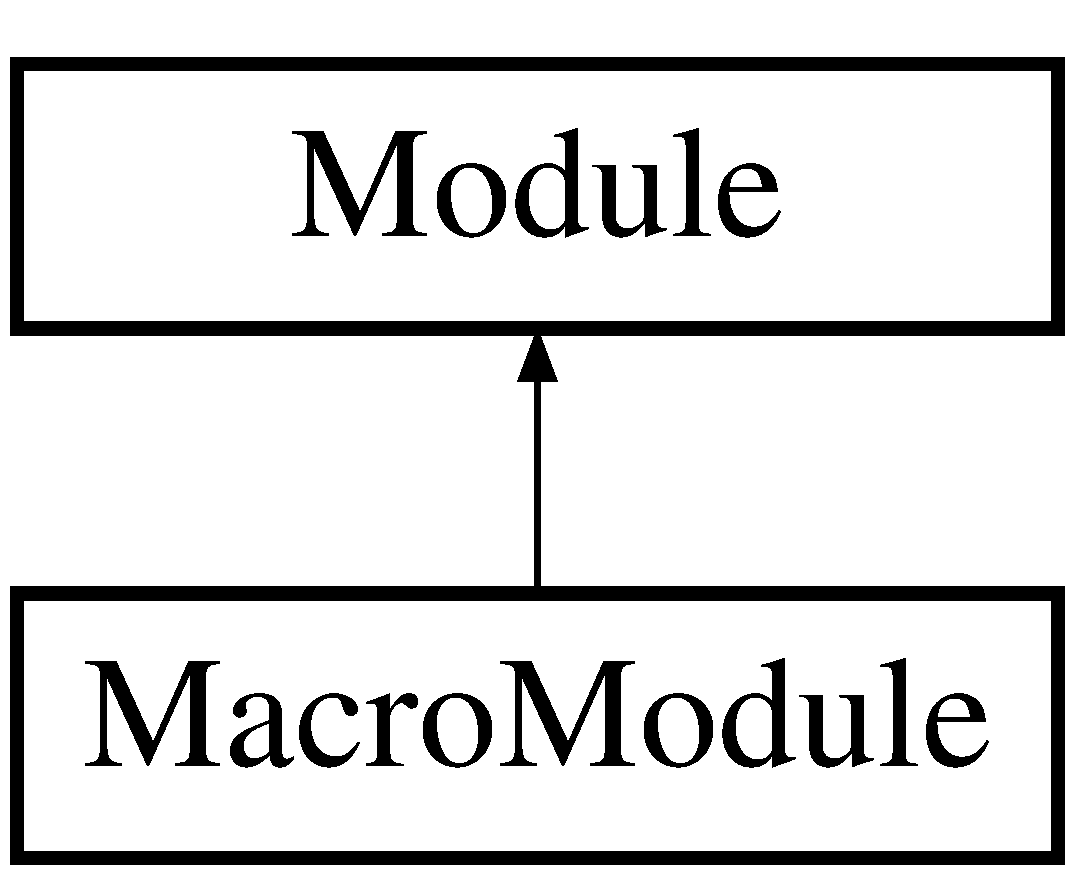
\includegraphics[height=2.000000cm]{classMacroModule}
\end{center}
\end{figure}
\subsection*{Fonctions membres publiques}
\begin{DoxyCompactItemize}
\item 
\hypertarget{classMacroModule_a9127bbdf48fc8088284daca146ec3143}{\hyperlink{classMacroModule_a9127bbdf48fc8088284daca146ec3143}{Macro\-Module} ()}\label{classMacroModule_a9127bbdf48fc8088284daca146ec3143}

\begin{DoxyCompactList}\small\item\em Constructeur. \end{DoxyCompactList}\item 
\hypertarget{classMacroModule_ae89dde4614b49decad95bbdebdefb0a2}{{\bfseries Macro\-Module} (\hyperlink{classMemory}{Memory}$<$ int $>$)}\label{classMacroModule_ae89dde4614b49decad95bbdebdefb0a2}

\item 
\hypertarget{classMacroModule_a9790fb7c331d99dd03f624b1a5258519}{\hyperlink{classMacroModule_a9790fb7c331d99dd03f624b1a5258519}{$\sim$\-Macro\-Module} ()}\label{classMacroModule_a9790fb7c331d99dd03f624b1a5258519}

\begin{DoxyCompactList}\small\item\em Destructeur. \end{DoxyCompactList}\item 
\hypertarget{classMacroModule_ab06c8308028b56ed94b599ed814a1864}{void {\bfseries add\-Sub\-Module} (\hyperlink{classModule}{Module})}\label{classMacroModule_ab06c8308028b56ed94b599ed814a1864}

\item 
\hypertarget{classMacroModule_ad5aca9e5f7b8784959dae226f845cd20}{void {\bfseries add\-Connexion} (\hyperlink{classConnexion}{Connexion})}\label{classMacroModule_ad5aca9e5f7b8784959dae226f845cd20}

\end{DoxyCompactItemize}


La documentation de cette classe a été générée à partir des fichiers suivants \-:\begin{DoxyCompactItemize}
\item 
src/headers/Macro\-Module.\-h\item 
src/includes/Macro\-Module.\-cpp\end{DoxyCompactItemize}

\hypertarget{classMemory}{\section{Référence de la classe Memory}
\label{classMemory}\index{Memory@{Memory}}
}


Repr�sente une m�moire.  




{\ttfamily \#include $<$Memory.\-h$>$}

\subsection*{Fonctions membres publiques}
\begin{DoxyCompactItemize}
\item 
\hypertarget{classMemory_a585d7bb6fc6f2237bcebf94a86b7dd99}{\hyperlink{classMemory_a585d7bb6fc6f2237bcebf94a86b7dd99}{Memory} ()}\label{classMemory_a585d7bb6fc6f2237bcebf94a86b7dd99}

\begin{DoxyCompactList}\small\item\em Constructeur. \end{DoxyCompactList}\item 
\hypertarget{classMemory_a0ffa9759ebbf103f11132a505b93bdc0}{\hyperlink{classMemory_a0ffa9759ebbf103f11132a505b93bdc0}{$\sim$\-Memory} ()}\label{classMemory_a0ffa9759ebbf103f11132a505b93bdc0}

\begin{DoxyCompactList}\small\item\em Destructeur. \end{DoxyCompactList}\end{DoxyCompactItemize}


\subsection{Description détaillée}
Repr�sente une m�moire. 

La m�moire est ici simplement mod�lis�e comme une liste de cl�es et de valeurs, associ�e � des contraintes. 

La documentation de cette classe a été générée à partir des fichiers suivants \-:\begin{DoxyCompactItemize}
\item 
src/headers/Memory.\-h\item 
src/includes/Memory.\-cpp\end{DoxyCompactItemize}

\hypertarget{classMessage}{\section{Référence de la classe Message}
\label{classMessage}\index{Message@{Message}}
}


Classe abstraite de base pour les messages.  




{\ttfamily \#include $<$Message.\-h$>$}

\subsection*{Fonctions membres publiques}
\begin{DoxyCompactItemize}
\item 
\hypertarget{classMessage_a4fc4f717b634e66070366cb7722d7761}{\hyperlink{classMessage_a4fc4f717b634e66070366cb7722d7761}{Message} ()}\label{classMessage_a4fc4f717b634e66070366cb7722d7761}

\begin{DoxyCompactList}\small\item\em Constructeur. \end{DoxyCompactList}\item 
\hypertarget{classMessage_a3f7275462831f787a861271687bcad67}{virtual \hyperlink{classMessage_a3f7275462831f787a861271687bcad67}{$\sim$\-Message} ()}\label{classMessage_a3f7275462831f787a861271687bcad67}

\begin{DoxyCompactList}\small\item\em Destructeur. \end{DoxyCompactList}\end{DoxyCompactItemize}


\subsection{Description détaillée}
Classe abstraite de base pour les messages. 

Les messages sont les différentes informations que peuvent se communiquer les modules. 

La documentation de cette classe a été générée à partir des fichiers suivants \-:\begin{DoxyCompactItemize}
\item 
src/headers/Message.\-h\item 
src/includes/Message.\-cpp\end{DoxyCompactItemize}

\hypertarget{classModule}{\section{Référence de la classe Module}
\label{classModule}\index{Module@{Module}}
}


Les briques de base du simulateur.  




{\ttfamily \#include $<$Module.\-h$>$}

\subsection*{Fonctions membres publiques}
\begin{DoxyCompactItemize}
\item 
\hypertarget{classModule_a5a240a8a9ab1813b17bcb810b24ceaea}{\hyperlink{classModule_a5a240a8a9ab1813b17bcb810b24ceaea}{Module} ()}\label{classModule_a5a240a8a9ab1813b17bcb810b24ceaea}

\begin{DoxyCompactList}\small\item\em Constructeur. \end{DoxyCompactList}\item 
\hypertarget{classModule_a7c9d9c096786d127590fdd8aa2b7d681}{virtual \hyperlink{classModule_a7c9d9c096786d127590fdd8aa2b7d681}{$\sim$\-Module} ()}\label{classModule_a7c9d9c096786d127590fdd8aa2b7d681}

\begin{DoxyCompactList}\small\item\em Destructeur. \end{DoxyCompactList}\end{DoxyCompactItemize}


\subsection{Description détaillée}
Les briques de base du simulateur. 

Il s'agit de la classe centrale du simulateur, qui sera construit comme un assemblage de modules qui communiquent entre eux. Il s'agit d'une classe virtuelle. 

La documentation de cette classe a été générée à partir des fichiers suivants \-:\begin{DoxyCompactItemize}
\item 
src/headers/Module.\-h\item 
src/includes/Module.\-cpp\end{DoxyCompactItemize}

\hypertarget{classNumberGeneratorModule}{\section{Référence de la classe Number\-Generator\-Module}
\label{classNumberGeneratorModule}\index{Number\-Generator\-Module@{Number\-Generator\-Module}}
}
Graphe d'héritage de Number\-Generator\-Module\-:\begin{figure}[H]
\begin{center}
\leavevmode
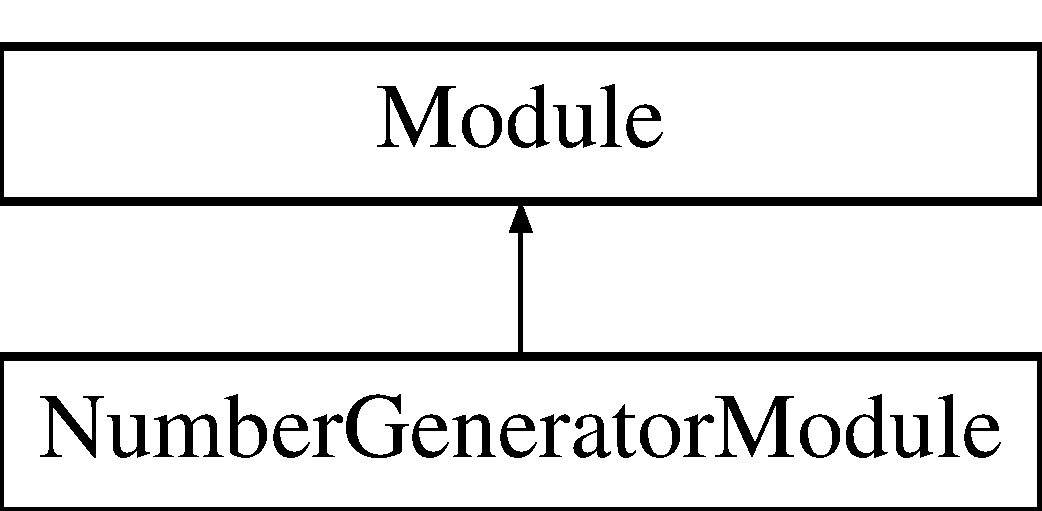
\includegraphics[height=2.000000cm]{classNumberGeneratorModule}
\end{center}
\end{figure}
\subsection*{Additional Inherited Members}


La documentation de cette classe a été générée à partir des fichiers suivants \-:\begin{DoxyCompactItemize}
\item 
src/headers/Number\-Generator\-Module.\-h\item 
src/includes/Number\-Generator\-Module.\-cpp\end{DoxyCompactItemize}

\hypertarget{classSocket}{\section{Référence de la classe Socket}
\label{classSocket}\index{Socket@{Socket}}
}


Classe abstraite pour les connecteurs des modules.  




{\ttfamily \#include $<$Socket.\-h$>$}

\subsection*{Types publics}
\begin{DoxyCompactItemize}
\item 
enum {\bfseries stype} \{ {\bfseries I\-N}, 
{\bfseries O\-U\-T}
 \}
\end{DoxyCompactItemize}
\subsection*{Fonctions membres publiques}
\begin{DoxyCompactItemize}
\item 
\hypertarget{classSocket_a008135f0646e48310061fe84b078dc81}{\hyperlink{classSocket_a008135f0646e48310061fe84b078dc81}{Socket} (std\-::string name, stype type)}\label{classSocket_a008135f0646e48310061fe84b078dc81}

\begin{DoxyCompactList}\small\item\em Constructeur. \end{DoxyCompactList}\item 
\hypertarget{classSocket_aeac4eb6379a543d38ed88977d3b6630a}{\hyperlink{classSocket_aeac4eb6379a543d38ed88977d3b6630a}{$\sim$\-Socket} ()}\label{classSocket_aeac4eb6379a543d38ed88977d3b6630a}

\begin{DoxyCompactList}\small\item\em Destructeur. \end{DoxyCompactList}\end{DoxyCompactItemize}


\subsection{Description détaillée}
Classe abstraite pour les connecteurs des modules. 

Les sockets modélisent les connections entre les modules. Un connecteur peut-\/être soit un connecteur d'entrée, {\itshape In\-Socket}, soit un connecteur de sortie, {\itshape Out\-S\-Ocket}. Les connecteurs sont reliés entre-\/eux via les objets \hyperlink{classConnexion}{Connexion}. 

La documentation de cette classe a été générée à partir des fichiers suivants \-:\begin{DoxyCompactItemize}
\item 
src/headers/Socket.\-h\item 
src/includes/Socket.\-cpp\end{DoxyCompactItemize}

\printindex
\end{document}
